\section{Background}

\subsection{Property Graph Model}

Graph databases are commonly based on the property graph model \cite{angles2018property}. A property graph is a directed, labeled multigraph in which both nodes and edges may carry labels and key-value properties.

Formally, a property graph is defined as a tuple
$G = (N, E, \rho, \lambda, \sigma)$,
where $N$ is the set of nodes, $E$ is the set of edges, $\rho$ defines edge connectivity, $\lambda$ assigns labels, and $\sigma$ defines property mappings \cite{angles2018property}. A path can be represented visually as shown in Figure 2.

\begin{figure}[ht]
    \centering
    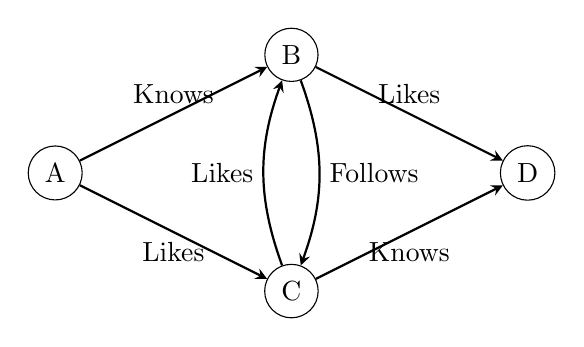
\begin{tikzpicture}[>=stealth]

        % Nodes
        \node[draw, circle] (A) at (0,0) {A};
        \node[draw, circle] (B) at (3,1.5) {B};
        \node[draw, circle] (C) at (3,-1.5) {C};
        \node[draw, circle] (D) at (6,0) {D};

        % Edges
        \draw[->, thick] (A) -- node[above] {Knows} (B);
        \draw[->, thick] (A) -- node[below] {Likes} (C);
        \draw[->, thick] (B) -- node[above] {Likes} (D);
        \draw[->, thick] (C) -- node[below] {Knows} (D);
        \draw[->, thick, bend left=20] (B) to node[right] {Follows} (C);
        \draw[->, thick, bend left=20] (C) to node[left] {Likes} (B);

    \end{tikzpicture}
    \caption{Simple Property Graph Model Illustration}
\end{figure}

\subsection{Paths in Graphs}

A path in a property graph is a sequence of alternating nodes and edges

\[
p = (n_1, e_1, n_2, \dots, e_k, n_{k+1})
\]

such that each edge connects consecutive nodes. Paths may be classified as walks, trails, acyclic paths, or simple paths depending on whether nodes or edges may repeat, as seem in the table below.

Path queries aim to retrieve sets of such paths satisfying structural or label constraints.


\begin{table}[ht]
    \centering
    \begin{tabular}{|l|p{7.5cm}|p{3.2cm}|}
        \hline
        \textbf{Path Type} & \textbf{Description} & \textbf{Example} \\
        \hline
        Walk &
        A path in which nodes and edges may be repeated.
        &
        A $\rightarrow$ B $\rightarrow$ C $\rightarrow$ B $\rightarrow$ D
        \\
        \hline
        Trail &
        A path in which no edge is repeated.
        &
        A $\rightarrow$ B $\rightarrow$ C $\rightarrow$ D
        \\
        \hline
        Acyclic &
        A path in which no node is repeated.
        &
        A $\rightarrow$ B $\rightarrow$ C $\rightarrow$ D
        \\
        \hline
        Simple &
        A path in which no node is repeated, except that the first and last nodes may be the same.
        &
        A $\rightarrow$ B $\rightarrow$ C $\rightarrow$ A
        \\
        \hline
    \end{tabular}
    \caption{Path semantics used in graph query languages \cite{angles2024path}.}
\end{table}

%}

\subsection{Graph Query Languages}

Modern graph query languages such as Cypher, SPARQL, SQL/PGQ, and GQL support path-oriented queries based on regular expressions over edge labels \cite{angles2017foundations,angles2024path}.

In contrast to classical RPQs, these languages aim to return not only reachable node pairs but also the actual witness paths. To control the potentially infinite number of such paths in cyclic graphs, GQL and SQL/PGQ introduce selectors and restrictors, which determine how paths are filtered and how recursion is interpreted \cite{angles2024path}.


\textbf{Example Queries:}

\begin{itemize}

    \item \textbf{Cypher and GQL} -- Matches a \texttt{KNOWS} relationship and returns the path.
\begin{verbatim}
MATCH p = (x)-[:KNOWS]->(y)
RETURN p
\end{verbatim}

    \item \textbf{SQL/PGQ} -- Matches a \texttt{KNOWS} relationship and returns the path.
\begin{verbatim}
SELECT p
FROM GRAPH_TABLE (
  my_graph
  MATCH p = (x)-[:KNOWS]->(y)
  COLUMNS (p)
)
\end{verbatim}

\end{itemize}
%}